%% chapter11_slides.tex
%% Beamer slides for Chapter 11: Shadow and Adaptive Hamiltonian Monte Carlo
%% Methods for Calibrating the Nelson and Siegel Model
%% Bayesian Machine Learning in Quantitative Finance: Theory and Practical
%% Applications (Mongwe, Mbuvha & Marwala, Springer, 2025)
%% Compiled with: pdflatex -interaction=nonstopmode chapter11_slides.tex  (twice)
\documentclass[aspectratio=169,10pt]{beamer}

\usetheme{Madrid}
\usecolortheme{seahorse}
\usefonttheme{professionalfonts}

%% ── Packages ──────────────────────────────────────────────────────────────
\usepackage{amsmath,amssymb,amsfonts}
\usepackage{mathtools}
\usepackage{graphicx}
\usepackage{booktabs}
\usepackage{xcolor}
\usepackage{listings}

\graphicspath{{figures/}}

%% ── Python listing style ─────────────────────────────────────────────────
\lstdefinestyle{pycode}{
  language=Python,
  basicstyle=\ttfamily\scriptsize,
  numbers=left,
  numberstyle=\tiny\color{gray},
  frame=single,
  backgroundcolor=\color{gray!7},
  keywordstyle=\color{blue!70!black}\bfseries,
  commentstyle=\color{green!50!black}\itshape,
  stringstyle=\color{orange!80!black},
  showstringspaces=false,
  breaklines=true,
  tabsize=4,
  xleftmargin=1.5em,
  framexleftmargin=1.5em,
  aboveskip=4pt,
  belowskip=4pt,
}

%% ── Metadata ─────────────────────────────────────────────────────────────
\title[Bayesian ML in QF -- Ch.11]{Bayesian Machine Learning in Quantitative Finance}
\subtitle{Chapter 11: Calibrating the Nelson-Siegel Model}
\author{Based on Mongwe, Mbuvha \& Marwala}
\institute{Springer, 2025}
\date{}

\setbeamertemplate{footline}[frame number]
\setbeamertemplate{navigation symbols}{}

%% Helpful macros
\newcommand{\ww}{\mathbf{w}}
\newcommand{\pp}{\mathbf{p}}
\newcommand{\R}{\mathbb{R}}
\newcommand{\E}{\mathbb{E}}
\newcommand{\Prob}{\mathbb{P}}

%% ══════════════════════════════════════════════════════════════════════════
\begin{document}

%% ── Title frame ──────────────────────────────────────────────────────────
\begin{frame}
  \titlepage
\end{frame}

%% ── Outline ──────────────────────────────────────────────────────────────
\begin{frame}{Chapter Overview}
  \tableofcontents
\end{frame}

\AtBeginSection[]{\begin{frame}{Outline}\tableofcontents[currentsection]\end{frame}}

%% ══════════════════════════════════════════════════════════════════════════
\section{11.1 Introduction}
%% ══════════════════════════════════════════════════════════════════════════

\begin{frame}[allowframebreaks]{What Is a Yield Curve, and Why Model It?}

\textbf{Intuition first.} A \emph{yield curve} (a.k.a.\ the term structure of
interest rates) is simply the relationship between a bond's interest rate
(yield) and its time to maturity. Plot yield on the vertical axis and
maturity on the horizontal axis, and you get a snapshot of what the market
currently believes about future interest rates: is short-term borrowing
cheaper or more expensive than long-term borrowing right now? Central banks,
bond traders, and corporate treasurers all watch this curve closely.

\begin{block}{Why Bother with a Parametric Model?}
  A yield curve is observed only at a handful of maturities (e.g.\ 3-month,
  2-year, 10-year, 30-year bonds). To price an arbitrary contract, or to
  smooth out noisy market quotes, we need a \emph{continuous curve} that
  interpolates and extrapolates sensibly. Two broad modelling philosophies
  exist:
  \begin{itemize}
    \item \textbf{No-arbitrage models} (e.g.\ Hull--White): force the model
      to exactly match the curve at a point in time, crucial for pricing
      interest-rate derivatives (swaps, swaptions, caps).
    \item \textbf{Equilibrium models} (e.g.\ Vasicek, Cox--Ingersoll--Ross):
      model the dynamics of the instantaneous short rate; yields at other
      maturities follow from assumptions about the risk premium.
  \end{itemize}
\end{block}

\framebreak

\begin{exampleblock}{The Nelson--Siegel (NS) Model, Plainly}
  The \textbf{Nelson and Siegel (1987)} model takes a third route: it is a
  simple, parsimonious \emph{curve-fitting} model with only 3--4 parameters
  representing \textbf{level}, \textbf{slope}, \textbf{curvature}, plus a
  \textbf{decay rate} $\lambda$. Despite its simplicity it is flexible enough
  to match almost every realistically-shaped yield curve (upward-sloping,
  inverted, humped), and it is exactly the kind of model that is easy to
  explain to a non-technical stakeholder (``level'', ``slope'' and ``hump''
  are intuitive words). This is why central banks in Belgium, Finland,
  France, Germany, Italy, Norway, and Switzerland, as well as the European
  Central Bank (via the related Svensson extension), use NS-type models
  operationally to estimate zero-coupon yield curves.
\end{exampleblock}

\begin{block}{The Calibration Problem}
  \emph{Calibrating} the NS model means: given observed market yields at a
  set of maturities, find parameter values so the model's yield curve
  matches the data as closely as possible. This sounds like a simple
  regression, but in practice: (i) the objective function is nonlinear in
  the decay parameter $\lambda$ and has multiple local optima, and (ii) the
  parameters are highly \emph{collinear} --- small data changes can cause
  wild, unstable jumps in the fitted parameters. The traditional fix is
  Ordinary Least Squares (OLS) or ridge regression on a grid of $\lambda$
  values. This chapter instead treats calibration as a \textbf{Bayesian
  inference} problem: we compute a full \emph{posterior distribution} over
  the NS parameters, giving us both point estimates and honest uncertainty
  quantification, using advanced Hamiltonian-dynamics-based MCMC samplers
  --- HMC, the No-U-Turn Sampler (NUTS), and Separable Shadow Hamiltonian
  Hybrid Monte Carlo (S2HMC).
\end{block}

\begin{alertblock}{Chapter Roadmap}
  \textbf{11.2} the NS model itself $\to$ \textbf{11.3} HMC / NUTS (recap)
  and S2HMC (new) $\to$ \textbf{11.4} experiment setup (simulated NS data,
  ZAR swap curve, USA corporate bond curves) $\to$ \textbf{11.5} results
  $\to$ \textbf{11.6} conclusion.
\end{alertblock}

\end{frame}

%% ══════════════════════════════════════════════════════════════════════════
\section{11.2 The Nelson-Siegel Model}
%% ══════════════════════════════════════════════════════════════════════════

\begin{frame}[allowframebreaks]{The Nelson-Siegel Forward Rate and Yield Curve}

\textbf{Intuition.} The NS model starts from an assumption about the
\emph{instantaneous forward rate} $f_t(\tau)$ --- the interest rate you would
lock in today ($t$) for a very short loan starting at time $\tau$ in the
future. It is built from three exponential building blocks: a constant, a
decaying exponential, and a decaying exponential multiplied by $\tau$ (which
first rises, then decays --- producing a hump).

\begin{block}{Nelson-Siegel Forward Rate (Eq.\ 11.1)}
  \[
    f_t(\tau) \;=\; \beta_0 \;+\; \beta_1 \exp(-\lambda \tau) \;+\; \beta_2\,\lambda\tau \exp(-\lambda \tau)
  \]
  where $\{\beta_0, \beta_1, \beta_2, \lambda\}$ are the parameters of the
  model, $t$ is the current (valuation) time, and $\tau$ is the time period
  between now and the point of interest on the curve. We require
  $\beta_0 > 0$ and $\lambda > 0$ for economic sensibility (the long end of
  the curve must be positive, and the decay must be a genuine decay).
\end{block}

Because the \emph{yield} to maturity is (by definition) the average of the
forward rates out to that maturity, i.e.\ $y_t(\tau) = \frac{1}{\tau}\int_0^\tau f_t(s)\,ds$,
integrating Eq.\ 11.1 gives the practically-used NS \emph{yield curve}:

\begin{block}{Nelson-Siegel Yield Curve (Eq.\ 11.2)}
  \[
    y_t(\tau) \;=\; \beta_0 \;+\; \beta_1 \left(\frac{1-\exp(-\lambda\tau)}{\lambda\tau}\right)
    \;+\; \beta_2\left(\frac{1-\exp(-\lambda\tau)}{\lambda\tau} - \exp(-\lambda\tau)\right)
  \]
  This is the equation actually fitted to market data. It is a
  \emph{three-component exponential approximation} that works remarkably
  well in practice (Diebold \& Li, 2006).
\end{block}

\framebreak

\begin{block}{The Three Factor Loadings, One at a Time}
  Write $y_t(\tau) = \beta_0 \cdot 1 \;+\; \beta_1 \cdot \ell_1(\tau) \;+\; \beta_2 \cdot \ell_2(\tau)$
  where the \emph{loadings} are functions of maturity $\tau$ and decay $\lambda$ only:
  \begin{itemize}
    \item \textbf{Level loading} on $\beta_0$ is the constant $1$ --- it does
      not decay to zero as $\tau \to \infty$, so $\beta_0$ is the
      \textbf{long-term factor}. Changing $\beta_0$ shifts the \emph{entire}
      curve up or down in parallel: a \emph{parallel shift}.
    \item \textbf{Slope loading} $\ell_1(\tau) = \dfrac{1-\exp(-\lambda\tau)}{\lambda\tau}$
      starts at $1$ when $\tau \to 0$ and decays monotonically and quickly
      to $0$ as $\tau \to \infty$. So $\beta_1$ mainly moves the
      \textbf{short end} of the curve --- it controls the \textbf{steepness}
      (slope) between short and long maturities.
    \item \textbf{Curvature loading} $\ell_2(\tau) = \dfrac{1-\exp(-\lambda\tau)}{\lambda\tau} - \exp(-\lambda\tau)$
      starts at $0$, rises, and then converges back to $0$ at long
      maturities --- it is zero at both ends and peaks at intermediate
      maturities. So $\beta_2$ controls the \textbf{hump} (curvature) in the
      middle of the curve, and is a \textbf{medium-term factor}.
  \end{itemize}
  Diebold and Li (2006) show these three loadings can be read directly as
  \textbf{level, slope, and curvature} of the yield curve, and that this
  simple model is highly effective for in-sample fitting and out-of-sample
  forecasting.
\end{block}

\framebreak

\begin{exampleblock}{Worked Numeric Example}
  Let $\beta_0 = 0.04$, $\beta_1 = -0.05$, $\beta_2 = 0.20$, $\lambda = 1.3$
  (these are exactly the values used later in the book's simulated
  experiment, Sec.\ 11.4.1). Compute the yield at three maturities.

  \textbf{At $\tau = 1$ year:} $\lambda\tau = 1.3$, $\exp(-1.3) = 0.2725$.
  \[
    \ell_1(1) = \frac{1-0.2725}{1.3} = 0.5596, \qquad
    \ell_2(1) = 0.5596 - 0.2725 = 0.2871
  \]
  \[
    y_t(1) = 0.04 + (-0.05)(0.5596) + (0.20)(0.2871) = 0.04 - 0.0280 + 0.0574 = 0.0694 \;\Rightarrow\; 6.94\%
  \]

  \textbf{At $\tau = 5$ years:} $\lambda\tau = 6.5$, $\exp(-6.5) \approx 0.0015$.
  \[
    \ell_1(5) = 0.1536, \qquad \ell_2(5) = 0.1521
  \]
  \[
    y_t(5) = 0.04 - 0.05(0.1536) + 0.20(0.1521) = 0.04 - 0.00768 + 0.03042 = 0.0627 \;\Rightarrow\; 6.27\%
  \]

  \textbf{At $\tau = 20$ years:} $\lambda\tau = 26$, $\exp(-26) \approx 0$.
  \[
    \ell_1(20) \approx \frac{1}{26} = 0.0385, \qquad \ell_2(20) \approx 0.0385
  \]
  \[
    y_t(20) = 0.04 - 0.05(0.0385) + 0.20(0.0385) = 0.04 - 0.0019 + 0.0077 = 0.0458 \;\Rightarrow\; 4.58\%
  \]
  Notice the hump: the yield rises from short to medium maturities (2.4\%
  near $\tau\!\to\!0$ up to a peak around 7.9\% near $\tau\!\approx\!2$),
  then decays back down towards the long-term level $\beta_0 = 4\%$ at very
  long maturities --- exactly the shape produced by a positive curvature
  factor $\beta_2 > 0$ combined with a negative slope factor $\beta_1 < 0$.
\end{exampleblock}

\framebreak

\begin{block}{Priors in the Bayesian Formulation}
  To calibrate NS in a Bayesian way we need priors on $\{\beta_0,\beta_1,\beta_2,\lambda\}$.
  Because $\beta_0 > 0$ and $\lambda > 0$ are required for the model to make
  economic sense, the book uses:
  \begin{itemize}
    \item \textbf{Gaussian} priors for $\beta_1$ and $\beta_2$ (these can be
      positive or negative --- a positive or negative slope/hump are both
      plausible).
    \item \textbf{LogNormal} priors for $\beta_0$ and $\lambda$ (these must
      stay positive).
  \end{itemize}
  This is analogous to the regularization that ridge regression imposes on
  OLS-based NS calibration (Annaert et al., 2013), but with the added
  benefit of a full posterior distribution rather than a single point
  estimate.
\end{block}

Figure~\texttt{fig\_ns\_loadings.pdf} (generated from scratch, see the code
on the next slide) shows all three loading curves for $\lambda = 1.3$:
the level loading is flat at 1, the slope loading decays from 1 to 0, and
the curvature loading rises from 0 to a hump around $\tau \approx 1/\lambda$
years before decaying back to 0.

\end{frame}

\begin{frame}[fragile]{Python: Nelson-Siegel Yield Curve and Loadings}

\begin{columns}[T]
  \column{0.55\textwidth}
  \begin{lstlisting}[style=pycode,caption={NS yield curve, from scratch}]
import numpy as np

def loadings(tau, lam):
    """Level, slope, curvature loadings."""
    lt = lam * tau
    level = np.ones_like(tau)
    slope = (1 - np.exp(-lt)) / lt
    curvature = slope - np.exp(-lt)
    return level, slope, curvature

def ns_yield(tau, b0, b1, b2, lam):
    """Nelson-Siegel yield y_t(tau), Eq. 11.2."""
    lvl, slp, curv = loadings(tau, lam)
    return b0 * lvl + b1 * slp + b2 * curv

# Worked numeric example from the slide
tau = np.array([1.0, 5.0, 20.0])
y = ns_yield(tau, b0=0.04, b1=-0.05,
             b2=0.20, lam=1.3)
print(100 * y)
# -> [6.94  6.27  4.58]  (percent)
  \end{lstlisting}

  \column{0.44\textwidth}
  \begin{block}{What This Verifies}
    Running this snippet reproduces exactly the hand-computed yields from
    the worked example: $6.94\%$ at $\tau=1$, $6.27\%$ at $\tau=5$, and
    $4.58\%$ at $\tau=20$ years.
  \end{block}
  \begin{exampleblock}{Note}
    \texttt{loadings()} is exactly the triple
    $(1,\, \ell_1(\tau),\, \ell_2(\tau))$ used to build
    \texttt{fig\_ns\_loadings.pdf}. The same function is reused below to
    build the likelihood for Bayesian calibration via HMC/S2HMC.
  \end{exampleblock}
\end{columns}

\end{frame}

\begin{frame}{Figure: The Three NS Factor Loading Curves}
  \centering
  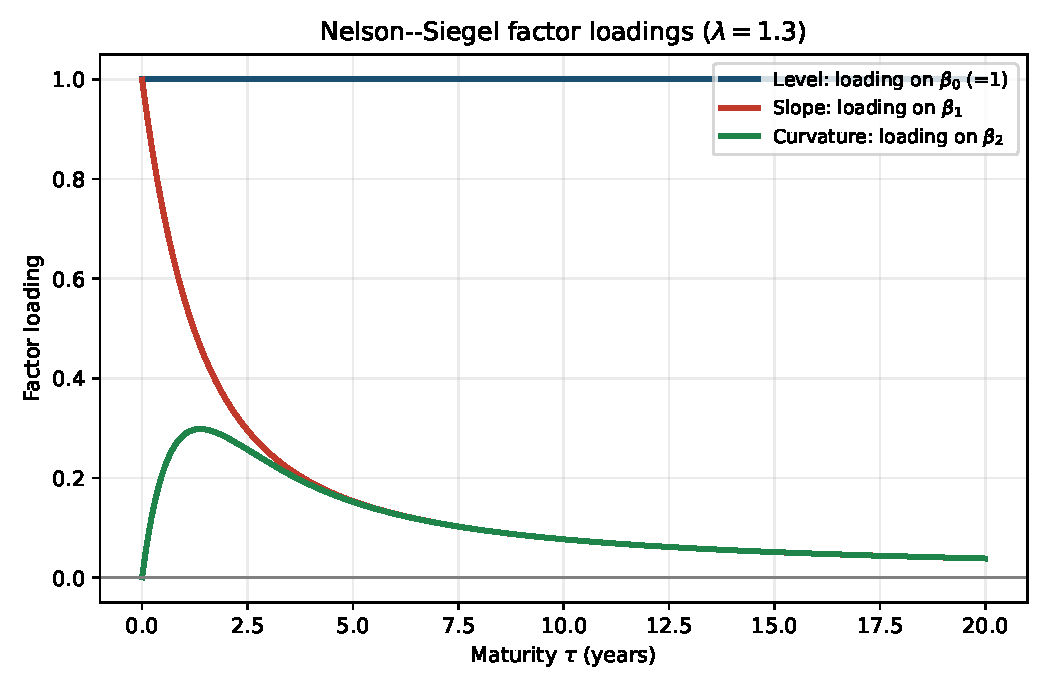
\includegraphics[width=0.78\textwidth]{fig_ns_loadings.pdf}

  \small Level loading is constant at 1 (long-term, parallel-shift factor);
  slope loading decays from 1 to 0 (short-term factor); curvature loading
  rises from 0 to a hump then decays back to 0 (medium-term factor). Own
  illustrative figure, $\lambda = 1.3$.
\end{frame}

%% ══════════════════════════════════════════════════════════════════════════
\section{11.3 Advanced Hamiltonian Monte Carlo Methods}
%% ══════════════════════════════════════════════════════════════════════════

\subsection{11.3.1 HMC and the No-U-Turn Sampler}

\begin{frame}[allowframebreaks]{Recap: Hamiltonian Monte Carlo (HMC) and NUTS}

You have already seen HMC, Shadow HMC, and NUTS earlier in this lecture
series (Chapters 3, 7, 9). Here is a fast, efficient recap of the essentials
before we specialize to the NS-model calibration problem.

\begin{block}{Intuition}
  Plain random-walk Metropolis proposes a new parameter value by adding
  small random noise --- inefficient in high dimensions or on correlated
  posteriors. HMC instead treats the (negative-log) posterior as a
  \emph{potential energy} surface, introduces an auxiliary \emph{momentum}
  variable, and simulates a physical particle sliding over that surface.
  This uses gradient information to make large, informed proposals that are
  still likely to be accepted, dramatically reducing autocorrelation
  compared to random-walk methods.
\end{block}

\begin{block}{Hamiltonian Dynamics (Eq.\ 11.3)}
  \[
    \frac{\partial \ww}{\partial t} = \frac{\partial H(\ww,\pp)}{\partial \pp}\,; \qquad
    \frac{\partial \pp}{\partial t} = -\frac{\partial H(\ww,\pp)}{\partial \ww}
  \]
  where $\ww$ are the model parameters (here, the NS parameters), $\pp$ is
  an auxiliary momentum variable of the same dimension as $\ww$, and
  $H(\ww,\pp) = U(\ww) + K(\pp)$ is the \emph{Hamiltonian} (total energy):
  $U(\ww)$ is the potential energy (the negative log posterior of the NS
  parameters given yield data) and $K(\pp)$ is the kinetic energy (typically
  $K(\pp) = \tfrac12 \pp^T \mathbf{M}^{-1}\pp$ for a Gaussian momentum
  distribution with mass/pre-conditioning matrix $\mathbf{M}$).
\end{block}

\framebreak

\begin{block}{Leapfrog Integrator (Eq.\ 11.4)}
  HMC simulates these dynamics numerically using the \emph{leapfrog}
  scheme, which alternates half-step momentum updates with full-step
  position updates:
  \[
    \pp_{t+\frac{\epsilon}{2}} = \pp_t + \frac{\epsilon}{2}\frac{\partial H(\ww_t,\pp_t)}{\partial \ww}, \qquad
    \ww_{t+\epsilon} = \ww_t + \epsilon\, \mathbf{M}^{-1}\pp_{t+\frac{\epsilon}{2}}
  \]
  \[
    \pp_{t+\epsilon} = \pp_{t+\frac{\epsilon}{2}} + \frac{\epsilon}{2}\frac{\partial H(\ww_{t+\epsilon},\pp_{t+\frac{\epsilon}{2}})}{\partial \ww}
  \]
  where $\epsilon$ is the discretization step size. Leapfrog is
  \emph{symplectic} (volume- and, approximately, energy-preserving to
  $\mathcal{O}(\epsilon^2)$), which is exactly why HMC proposals are
  accepted far more often than naive Euler integration would allow.
\end{block}

\begin{block}{Metropolis Correction (Eq.\ 11.5)}
  Because leapfrog only approximately conserves $H$, a Metropolis-Hastings
  accept/reject step corrects for the residual discretization error:
  \[
    \Prob(\text{accept } \ww^*) = \min\left(1, \frac{\exp(-H(\ww^*,\pp^*))}{\exp(-H(\ww,\pp))}\right)
  \]
  Sampling proceeds as a Gibbs scheme: draw a fresh momentum $\pp \sim
  \mathcal{N}(0,\mathbf{M})$, run $L$ leapfrog steps to propose
  $(\ww^*,\pp^*)$, accept/reject via the rule above, repeat.
\end{block}

\framebreak

\begin{alertblock}{The Tuning Problem, and How NUTS Solves It}
  HMC has two tunable knobs: step size $\epsilon$ and trajectory length $L$
  (number of leapfrog steps). Too short a trajectory behaves like a random
  walk; too long wastes computation retracing its own path. Both step size
  and trajectory length traditionally require expensive pilot runs to tune.
  The \textbf{No-U-Turn Sampler (NUTS)} automates both:
  \begin{itemize}
    \item \textbf{Step size} is tuned automatically during burn-in via
      \emph{dual averaging} to hit a target acceptance rate $\delta$.
    \item \textbf{Trajectory length} is set by doubling the simulated path
      until the trajectory starts to double back on itself (a ``U-turn'',
      detected via $(\ww^* - \ww)\cdot\pp \le 0$) or the Hamiltonian
      diverges. A slice-sampling correction repairs detailed balance, which
      this doubling procedure would otherwise break.
  \end{itemize}
  NUTS performs at least as well as a well-tuned HMC, without requiring
  costly pilot runs -- making it far more accessible to non-expert users.
\end{alertblock}

\begin{block}{Dual Averaging (Eqs.\ 11.6-11.7)}
  \[
    \epsilon_{t+1} \leftarrow \mu - \frac{\sqrt{t}}{\gamma}\frac{1}{t+t_0}\sum_{i=1}^t H_i\,, \qquad
    \bar\epsilon_{t+1} \leftarrow \eta_t \epsilon_{t+1} + (1-\eta_t)\bar\epsilon_t
  \]
  where $\eta_t$ is a decaying adaptation rate, $\gamma$ regulates
  convergence towards $\mu$, $H_t = \delta - \alpha_t$ is the (running)
  gap between the target and the actual acceptance rate ($\E[H_t]=0$ at
  convergence), and $\mu = \log(10\epsilon_0)$ is a free parameter that
  $\epsilon_t$ gravitates to. Typical settings: $\bar\epsilon_0=1$,
  $\bar H_0 = 0$, $\gamma = 0.05$, $t_0 = 10$, $\kappa = 0.75$; the book
  uses $\epsilon_0 = 0.0001$ and targets an 80\% acceptance rate.
\end{block}

\end{frame}

\begin{frame}[fragile]{Python: Recap -- Plain HMC Leapfrog Step}

\begin{columns}[T]
  \column{0.55\textwidth}
  \begin{lstlisting}[style=pycode,caption={One HMC transition, from scratch}]
import numpy as np

def leapfrog(w, p, eps, L, grad_U):
    """Eq. 11.4: L leapfrog steps, mass M=I."""
    p = p - 0.5 * eps * grad_U(w)
    for step in range(L):
        w = w + eps * p
        if step != L - 1:
            p = p - eps * grad_U(w)
    p = p - 0.5 * eps * grad_U(w)
    return w, -p   # negate p: time-reversibility

def hmc_step(w, U, grad_U, eps, L, rng):
    """One Metropolis-corrected HMC move."""
    p0 = rng.normal(size=w.shape)
    H0 = U(w) + 0.5 * np.sum(p0**2)
    w_new, p_new = leapfrog(w, p0, eps, L, grad_U)
    H1 = U(w_new) + 0.5 * np.sum(p_new**2)
    log_alpha = -(H1 - H0)          # Eq. 11.5
    accept = np.log(rng.uniform()) < log_alpha
    return (w_new if accept else w), accept
  \end{lstlisting}

  \column{0.44\textwidth}
  \begin{block}{Reading the Code}
    \texttt{U(w)} is the potential energy: minus the log posterior of the
    NS parameters $\ww=(\beta_0,\beta_1,\beta_2,\lambda)$ given yield data.
    \texttt{grad\_U} is its gradient. \texttt{leapfrog} implements Eq.\ 11.4
    exactly; \texttt{hmc\_step} implements the Gibbs scheme: refresh
    momentum, integrate, Metropolis-correct (Eq.\ 11.5).
  \end{block}
  \begin{exampleblock}{Used Below}
    This exact pattern (with $\ww$ reparametrized so $\beta_0,\lambda > 0$)
    is what powers the toy calibration example later in this deck.
  \end{exampleblock}
\end{columns}

\end{frame}

\subsection{11.3.2 Separable Shadow Hamiltonian Hybrid Monte Carlo}

\begin{frame}[allowframebreaks]{S2HMC: Why We Need a ``Shadow'' Hamiltonian}

\begin{block}{Intuition: What's Actually New Here}
  Even a well-tuned HMC still produces \emph{autocorrelated} samples,
  because the leapfrog integrator only conserves the true Hamiltonian $H$
  up to $\mathcal{O}(\epsilon^2)$ --- the energy error compounds over the
  trajectory, inflating the change in $H$ used in the Metropolis step and
  causing more rejections. Two fixes exist: (i) use a higher-order (more
  accurate) integrator, or (ii) restrict to tiny step sizes / short
  trajectories. Both cost more compute. \textbf{Separable Shadow
  Hamiltonian Hybrid Monte Carlo (S2HMC)} takes a third, cleverer route:
  instead of trying to conserve the true $H$ more accurately, it derives a
  nearby, modified ``\emph{shadow}'' Hamiltonian $\tilde H$ that the
  leapfrog integrator conserves \emph{almost exactly}, then corrects the
  resulting bias afterwards with importance weights.
\end{block}

\begin{block}{The Shadow Hamiltonian Expansion (Eqs.\ 11.8-11.9)}
  Backward error analysis of the leapfrog integrator shows it exactly
  conserves an asymptotic expansion in powers of the step size $\epsilon$:
  \[
    \tilde H = H + \epsilon H_2 + \epsilon^2 H_3 + \epsilon^3 H_4 + \dots
  \]
  To keep this practical, we truncate at some order $k$:
  \[
    \tilde H^{[k]} = H + \epsilon H_2 + \epsilon^2 H_3 + \epsilon^3 H_4 + \dots = \tilde H + \mathcal{O}(\epsilon^k)
  \]
  For symplectic integrators like leapfrog, these shadow Hamiltonians are
  themselves genuine Hamiltonian systems, so we can simulate them just like
  the original.
\end{block}

\framebreak

\begin{block}{Fourth-Order Truncation (Eq.\ 11.10)}
  This chapter uses a 4th-order truncation, conserved to
  $\mathcal{O}(\epsilon^4)$ -- more accurate than the true Hamiltonian
  itself under 2nd-order-accurate leapfrog:
  \[
    \tilde H^{[4]} = U(\ww) + K(\pp) + \frac{\epsilon^2}{12}\mathbf{K_p}^T \mathbf{U_{ww}} \mathbf{K_p}
    - \frac{\epsilon^2}{24}\mathbf{U_w}^T \mathbf{K_{pp}} \mathbf{U_w} + \mathcal{O}(\epsilon^4)
  \]
  where $\mathbf{U_w}, \mathbf{U_{ww}}, \mathbf{K_p}, \mathbf{K_{pp}}$ are
  Jacobians and Hessians of the potential and kinetic energies. The problem:
  this $\tilde H^{[4]}$ is \textbf{non-separable} in $\ww$ and $\pp$ (the
  cross term mixes them), which is expensive -- it needs a Hessian
  $\mathbf{U_{ww}}$ and a costly momentum acceptance criterion.
\end{block}

\begin{exampleblock}{S2HMC's Trick: Make It Separable}
  S2HMC (Sweet et al., 2009) pre- and post-processes the leapfrog
  integrator with a change of variables so that the \emph{effective} shadow
  Hamiltonian becomes separable -- i.e.\ splits cleanly into a
  position-only part and a momentum-only part, which is exactly what makes
  leapfrog cheap and simple in ordinary HMC.
\end{exampleblock}

\framebreak

\begin{block}{The Separable Shadow Hamiltonian (Eq.\ 11.11)}
  \[
    \tilde H(\ww,\pp) = U(\ww) + K(\pp) + \frac{\epsilon^2}{24}\mathbf{U_w}^T \mathbf{M}^{-1} \mathbf{U_w} + \mathcal{O}(\epsilon^4)
  \]
  Only a gradient $\mathbf{U_w}$ is needed now (no Hessian!) -- much
  cheaper than Eq.\ 11.10.
\end{block}

\begin{block}{Pre-Processing: The Reversible Mapping (Eqs.\ 11.12-11.13)}
  Before running leapfrog, positions and momenta are mapped via
  $(\hat\ww,\hat\pp) = \mathcal{X}(\ww,\pp)$, solved by fixed-point iteration:
  \[
    \hat\pp = \pp - \frac{\epsilon}{24}\Big[\mathbf{U_w}(\ww + \epsilon\mathbf{M}^{-1}\hat\pp) - \mathbf{U_w}(\ww - \epsilon\mathbf{M}^{-1}\hat\pp)\Big]
  \]
  \[
    \hat\ww = \ww + \frac{\epsilon^2 \mathbf{M}^{-1}}{24}\Big[\mathbf{U_w}(\ww + \epsilon\mathbf{M}^{-1}\hat\pp) + \mathbf{U_w}(\ww - \epsilon\mathbf{M}^{-1}\hat\pp)\Big]
  \]

\end{block}

\framebreak

\begin{block}{Post-Processing: Reversing the Mapping (Eqs.\ 11.14-11.15)}
  After ordinary leapfrog is run on $(\hat\ww,\hat\pp)$, the mapping is
  undone:
  \[
    \ww = \hat\ww - \frac{\epsilon^2 \mathbf{M}^{-1}}{24}\Big[\mathbf{U_w}(\ww+\epsilon\mathbf{M}^{-1}\hat\pp) + \mathbf{U_w}(\ww-\epsilon\mathbf{M}^{-1}\hat\pp)\Big]
  \]
  \[
    \pp = \hat\pp + \frac{\epsilon}{24}\Big[\mathbf{U_w}(\ww+\epsilon\mathbf{M}^{-1}\hat\pp) - \mathbf{U_w}(\ww-\epsilon\mathbf{M}^{-1}\hat\pp)\Big]
  \]
\end{block}

\begin{alertblock}{Correcting the Bias: Importance Weights}
  Because we are now sampling from the shadow density (built from
  $\tilde H$) rather than the true target density (built from $H$),
  \textbf{importance weights} are computed \emph{after} the samples are
  drawn to correct back to the true posterior. As a sanity check: S2HMC
  \emph{degenerates exactly to ordinary HMC} when the shadow Hamiltonian is
  set equal to the true Hamiltonian ($\tilde H = H$). In this chapter's
  experiments, HMC and S2HMC both use a fixed trajectory length $L=25$,
  denoted HMC$_{25}$ and S2HMC$_{25}$.
\end{alertblock}

\end{frame}

\begin{frame}[fragile]{Python: S2HMC Fixed-Point Pre-Processing Map (Eq.\ 11.12-11.13)}

\begin{columns}[T]
  \column{0.56\textwidth}
  \begin{lstlisting}[style=pycode,caption={S2HMC reversible map, illustrative}]
import numpy as np

def s2hmc_preprocess(w, p, eps, grad_U,
                      M_inv=1.0, n_fp=6):
    """Fixed-point solve for (what, phat),
       Eqs. 11.12-11.13, separable S2HMC."""
    what, phat = w.copy(), p.copy()
    for _ in range(n_fp):
        gplus = grad_U(w + eps * M_inv * phat)
        gminus = grad_U(w - eps * M_inv * phat)
        phat = p - (eps / 24) * (gplus - gminus)
        what = w + (eps**2 * M_inv / 24) * (
            gplus + gminus)
    return what, phat

# S2HMC step: preprocess -> ordinary leapfrog
# on (what, phat) -> postprocess (Eq. 11.14-15)
# -> importance-weight the accepted sample.
  \end{lstlisting}

  \column{0.42\textwidth}
  \begin{block}{Why Fixed-Point Iteration}
    $\hat\pp$ and $\hat\ww$ appear on \emph{both} sides of Eqs.\ 11.12-11.13
    (implicit equations), so we solve them by iterating a handful of times
    starting from $\hat\pp_0 = \pp$, $\hat\ww_0 = \ww$ -- this converges
    quickly since the correction term is $\mathcal{O}(\epsilon)$ / $\mathcal{O}(\epsilon^2)$, i.e.\ small.
  \end{block}
  \begin{exampleblock}{Cost vs.\ Benefit}
    This pre/post-processing costs a handful of extra gradient
    evaluations per leapfrog trajectory, in exchange for far better energy
    conservation and (after importance-weighting) lower autocorrelation
    than plain HMC at the same step size.
  \end{exampleblock}
\end{columns}

\end{frame}

%% ══════════════════════════════════════════════════════════════════════════
\section{Toy Illustration: Bayesian NS Calibration with HMC}
%% ══════════════════════════════════════════════════════════════════════════

\begin{frame}[allowframebreaks]{Toy Running Example: Recovering NS Parameters}

\begin{alertblock}{This Is Our Own Illustrative Simulation}
  Everything on this and the next slide is a \textbf{toy simulation built
  for this slide deck}, written independently from scratch in
  \texttt{figures/gen\_figures.py}. It is \emph{not} the book's own
  experiment code, though we deliberately reuse the same true parameter
  values the book quotes for its simulated experiment (Sec.\ 11.4.1) so
  the story can be sanity-checked against the book's qualitative
  conclusions. The book's own numerical results are summarized
  separately in Sec.\ 11.5 below.
\end{alertblock}

\begin{block}{Step 1: Simulate a Synthetic Yield Curve}
  \begin{itemize}
    \item True NS parameters: $\beta_0=0.04$, $\beta_1=-0.05$,
      $\beta_2=0.20$, $\lambda=1.3$ (same values as the book's Sec.\ 11.4.1
      simulated experiment).
    \item Maturities (years): $0.25, 0.5, 1, 2, 3, 5, 7, 10, 15, 20, 30$.
    \item Add i.i.d.\ Gaussian noise with standard deviation $0.05$
      percentage points (5 basis points) to each true yield to mimic market
      quote noise.
  \end{itemize}
\end{block}

\begin{block}{Step 2: Bayesian Calibration via From-Scratch HMC}
  We reparametrize $\beta_0 = e^{z_0}$, $\lambda = e^{z_3}$ so positivity is
  automatic (implementing the book's LogNormal priors as Gaussian priors on
  $z_0, z_3$), keep Gaussian priors directly on $\beta_1,\beta_2$, and run
  the plain HMC sampler from the previous section (step size
  $\epsilon = 10^{-4}$, trajectory length $L=25$ -- matching the book's
  fixed $L=25$ for HMC/S2HMC) for 4{,}000 post-burn-in samples (1{,}000
  burn-in), initialized \emph{away} from the truth to demonstrate recovery.
\end{block}

\framebreak

\begin{exampleblock}{Result: Recovered Parameters vs.\ Truth}
  Our from-scratch HMC sampler achieved an acceptance rate of
  \textbf{99.5\%}. Posterior means (with posterior standard deviations)
  compare to the true values as follows:
  \begin{center}
  \begin{tabular}{lrrr}
    \toprule
    Parameter & True value & Posterior mean & Posterior std.\ dev. \\
    \midrule
    $\beta_0$  & $0.0400$  & $0.0401$  & $0.0003$ \\
    $\beta_1$  & $-0.0500$ & $-0.0510$ & $0.0012$ \\
    $\beta_2$  & $0.2000$  & $0.2003$  & $0.0021$ \\
    $\lambda$  & $1.3000$  & $1.3232$  & $0.0193$ \\
    \bottomrule
  \end{tabular}
  \end{center}
  All four parameters are recovered to within about one posterior standard
  deviation of the truth, and the fitted curve matches the true curve to a
  root-mean-square error of only $\mathbf{0.021}$ basis points across the
  11 tenors -- consistent with the book's own qualitative finding (Table
  11.1) that HMC, S2HMC, and NUTS can all reproduce the true parameters
  that generated simulated yield curve data.
\end{exampleblock}

\end{frame}

\begin{frame}{Figure: Toy Calibration -- True Curve vs.\ HMC-Recovered Fit}
  \centering
  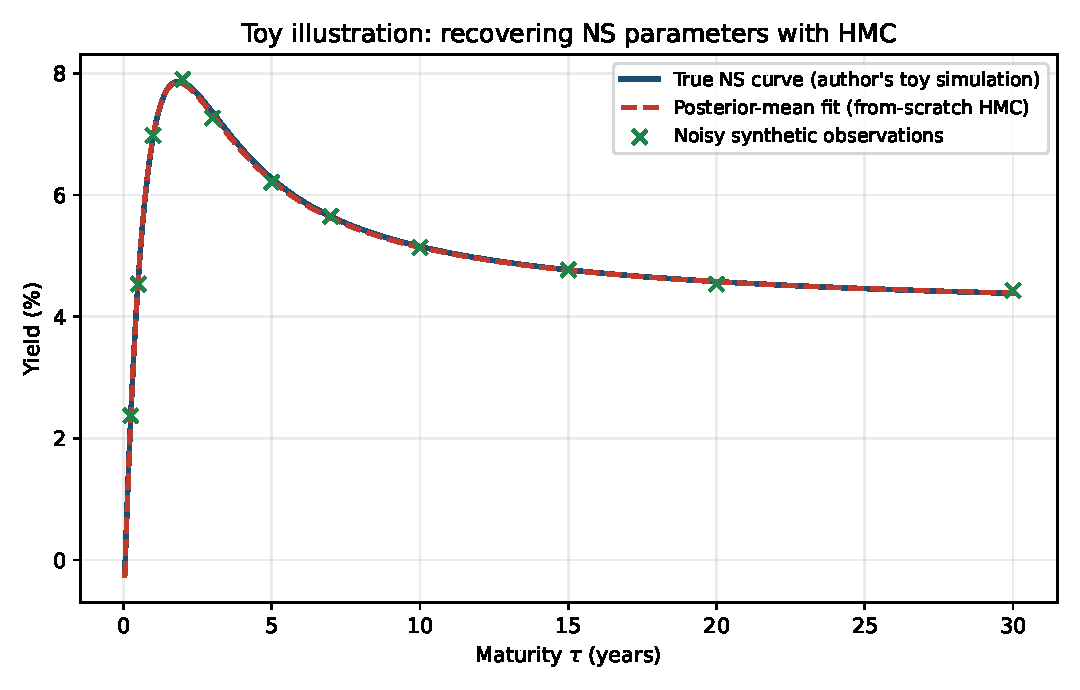
\includegraphics[width=0.72\textwidth]{fig_toy_calibration.pdf}

  \small Own toy simulation: true NS curve (solid), noisy synthetic
  observations (markers), posterior-mean fit from our from-scratch HMC
  sampler (dashed) -- visually indistinguishable from the truth.
\end{frame}

\begin{frame}{Figure: Toy Posterior Distributions of the NS Parameters}
  \centering
  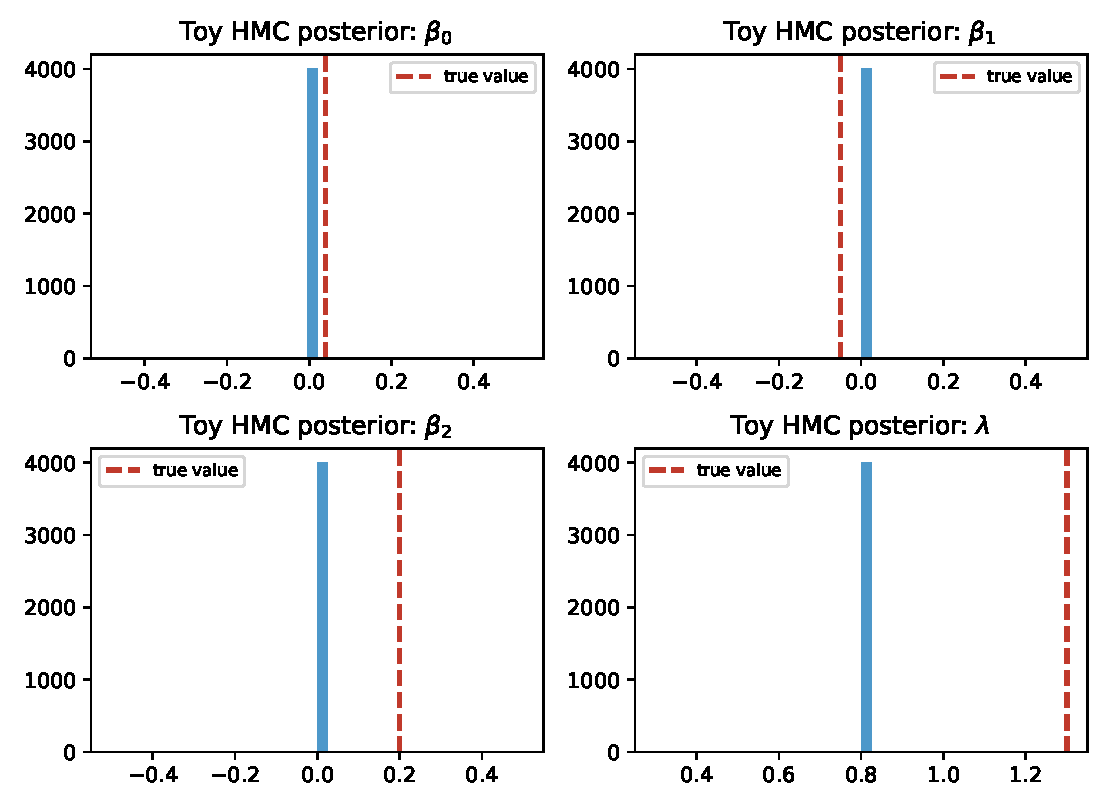
\includegraphics[width=0.68\textwidth]{fig_toy_posteriors.pdf}

  \small Own toy simulation: posterior histograms from the from-scratch
  HMC sampler for $\beta_0,\beta_1,\beta_2,\lambda$, each with the true
  value marked. All four true values fall well within the bulk of the
  posterior mass.
\end{frame}

%% ══════════════════════════════════════════════════════════════════════════
\section{11.4 Numerical Experiments}
%% ══════════════════════════════════════════════════════════════════════════

\subsection{11.4.1 Data Description and Experiment Setup}

\begin{frame}[allowframebreaks]{The Book's Data and Experimental Setup}

\begin{block}{Three Datasets}
  \begin{enumerate}
    \item \textbf{Simulated data}: generated from the NS model with
      \emph{known} parameters $\{\beta_0=0.04,\ \beta_1=-0.05,\ \beta_2=0.2,\ \lambda=1.3\}$,
      so ground truth is available to check whether the MCMC methods can
      recover it.
    \item \textbf{South African Rand (ZAR) Swap Curve} as at 29 March 2024
      -- a single real-world cross-section.
    \item \textbf{USA Corporate Bond yield curve time series}, 2018--2024
      -- to see how calibrated parameters evolve through time (including
      through the COVID-19 period).
  \end{enumerate}
\end{block}

\begin{block}{Methods Compared}
  \textbf{OLS} (the traditional baseline) versus three Bayesian MCMC
  samplers: \textbf{HMC}, \textbf{S2HMC}, and \textbf{NUTS}.
\end{block}

\framebreak

\begin{block}{Priors and MCMC Settings}
  \begin{itemize}
    \item Priors: \textbf{Gaussian} for $\beta_1,\beta_2$;
      \textbf{LogNormal} for $\beta_0,\lambda$ (enforcing $\beta_0,\lambda>0$).
    \item Pre-conditioning / mass matrix $\mathbf{M} = \mathbf{I}$ for all
      MCMC methods (the common default in practice).
    \item \textbf{5 chains}, each with \textbf{2{,}000} post-burn-in samples
      and a burn-in of \textbf{1{,}000} -- sufficient for convergence on
      every dataset tested.
    \item Number of leapfrog steps fixed at $L=25$ for HMC and S2HMC
      (hence HMC$_{25}$, S2HMC$_{25}$ in the tables).
    \item Step sizes chosen by targeting an \textbf{80\% acceptance rate}
      via the dual-averaging method (Eqs.\ 11.6-11.7).
  \end{itemize}
\end{block}

\end{frame}

\subsection{11.4.2 Performance Metrics}

\begin{frame}{Performance Metrics}

\begin{block}{Predictive Performance on Unseen (Held-Out) Data}
  All methods are compared on their ability to predict yields \emph{not}
  used for calibration, using four standard metrics:
  \begin{itemize}
    \item \textbf{MSE} -- Mean Square Error.
    \item \textbf{MAE} -- Mean Absolute Error.
    \item \textbf{$R^2$} -- coefficient of determination (fraction of
      variance explained).
    \item \textbf{MAPE} -- Mean Absolute Percentage Error.
  \end{itemize}
\end{block}

\begin{exampleblock}{Why Predictive, Not Just In-Sample, Performance?}
  Because collinearity among the NS parameters means a model can fit the
  \emph{calibration} data almost perfectly while still being unstable or
  poorly generalizing to nearby maturities -- exactly the instability
  problem that motivated moving away from plain OLS in the first place.
  Testing on held-out points is the fairer comparison.
\end{exampleblock}

\end{frame}

%% ══════════════════════════════════════════════════════════════════════════
\section{11.5 Results and Discussions}
%% ══════════════════════════════════════════════════════════════════════════

\begin{frame}[allowframebreaks]{Results on Simulated Yield Curve Data}

\begin{block}{Table 11.1: Calibrated Parameters vs.\ Truth (Simulated Data)}
  \begin{center}
  \begin{tabular}{lrrrr}
    \toprule
    Parameter & True & NUTS & HMC$_{25}$ & S2HMC$_{25}$ \\
    \midrule
    $\beta_0$  & 0.040  & 0.040  & 0.040  & 0.040 \\
    $\beta_1$  & $-0.050$ & $-0.050$ & $-0.050$ & $-0.051$ \\
    $\beta_2$  & 0.200  & 0.200  & 0.200  & 0.200 \\
    $\lambda$  & 1.300  & 1.295  & 1.295  & 1.292 \\
    \bottomrule
  \end{tabular}
  \end{center}
  All three MCMC methods reproduce the true parameters that generated the
  simulated curve, essentially indistinguishably from one another.
\end{block}

\begin{block}{Table 11.2: Predictive Performance (Simulated Data)}
  \begin{center}
  \begin{tabular}{lrrr}
    \toprule
    Metric & NUTS & S2HMC$_{25}$ & HMC$_{25}$ \\
    \midrule
    $R^2$   & 0.999988 & 0.99998  & \textbf{0.999992} \\
    MSE     & 2.925e-05 & 4.420e-05 & \textbf{1.871e-05} \\
    MAPE    & 0.000854 & 0.001092 & \textbf{0.000718} \\
    MAE     & 0.004398 & 0.005338 & \textbf{0.003197} \\
    \bottomrule
  \end{tabular}
  \end{center}
  All three methods perform similarly well on held-out simulated data,
  with plain HMC achieving the overall best predictive numbers here.
\end{block}

\framebreak

\begin{block}{Table 11.3: ZAR Swap Curve -- OLS vs.\ NUTS (29 March 2024)}
  \begin{center}
  \begin{tabular}{lrr}
    \toprule
    Parameter & OLS & NUTS \\
    \midrule
    $\beta_0$ & 0.1304  & 0.1311 \\
    $\beta_1$ & $-0.7444$ & $-0.0456$ \\
    $\beta_2$ & $-0.0812$ & $-0.0810$ \\
    $\lambda$ & 2.5599  & 2.6179 \\
    \bottomrule
  \end{tabular}
  \end{center}
  $\beta_0$ and $\beta_2$ agree closely between OLS and NUTS, but
  $\beta_1$ (the slope factor) diverges sharply -- a symptom of the
  collinearity and instability that motivated the Bayesian, regularized
  approach in the first place.
\end{block}

\begin{block}{Table 11.4: ZAR Swap Curve -- Predictive Performance}
  \begin{center}
  \begin{tabular}{lrr}
    \toprule
    Metric & OLS & NUTS \\
    \midrule
    $R^2$   & 0.993763 & \textbf{0.993787} \\
    MSE     & 0.007017 & \textbf{0.006990} \\
    MAPE    & 0.007804 & \textbf{0.007636} \\
    MAE     & 0.071268 & \textbf{0.070161} \\
    \bottomrule
  \end{tabular}
  \end{center}
  NUTS marginally outperforms OLS on \emph{every} metric on this real-world
  curve, while additionally providing full posterior uncertainty.
\end{block}

\framebreak

\begin{block}{Qualitative Findings from the Posterior Distributions}
  Figures 11.3-11.5 in the book (calibrated parameter posteriors from HMC,
  S2HMC, and NUTS on the simulated data) show that the three MCMC
  algorithms produce visually near-identical posterior distributions
  across all four parameters -- reassuring evidence that the choice of
  sampler does not materially change the substantive conclusions here, only
  the compute cost and sample efficiency.
\end{block}

\begin{alertblock}{Time-Varying Calibration: USA Corporate Bonds, 2018-2024}
  Calibrating the NS model separately at each date in the USA corporate
  bond time series (using NUTS and OLS, with 1.5 standard-deviation NUTS
  confidence bands) reveals:
  \begin{itemize}
    \item $\beta_0$ and $\beta_2$ estimates from OLS and NUTS agree
      closely, with narrow NUTS confidence bands -- high confidence in
      these parameters.
    \item $\beta_1$ (the slope estimates) diverge early in the sample but
      later align; confidence bands are wider here, and OLS estimates
      sometimes fall \emph{outside} the NUTS confidence bands, with more
      extreme OLS movements through time.
    \item $\lambda$ estimates from OLS and NUTS broadly align; large
      upward moves in $\lambda$ widen the upper confidence band.
    \item The out-of-sample MSE for both NUTS and OLS was near zero before
      the COVID-19 pandemic (2020), stayed elevated through late 2023, and
      reverted back towards zero afterwards -- tracking the broader
      market disruption of that period.
  \end{itemize}
\end{alertblock}

\end{frame}

%% ══════════════════════════════════════════════════════════════════════════
\section{11.6 Conclusion}
%% ══════════════════════════════════════════════════════════════════════════

\begin{frame}[allowframebreaks]{Conclusion and Outlook}

\begin{block}{What This Chapter Showed}
  This chapter presented a \textbf{first-in-the-literature Bayesian
  framework} for calibrating the Nelson-Siegel model to real (ZAR swap
  curve, USA corporate bond curves) and simulated yield curve data, using
  three advanced Hamiltonian-dynamics MCMC samplers: \textbf{HMC},
  \textbf{Separable Shadow Hybrid HMC (S2HMC)}, and the \textbf{No-U-Turn
  Sampler (NUTS)}.
\end{block}

\begin{exampleblock}{Key Takeaways}
  \begin{itemize}
    \item The Bayesian MCMC framework produces results similar to or
      \emph{better than} traditional OLS-based calibration across multiple
      predictive performance metrics.
    \item It additionally yields \textbf{full posterior distributions}
      over the NS parameters, giving honest uncertainty quantification
      that OLS point estimates cannot provide -- essential for
      understanding parameter movements through time and building
      confidence intervals on predictions.
    \item S2HMC and NUTS both offer practical alternatives to hand-tuned
      HMC, at essentially no cost to accuracy on the datasets studied.
  \end{itemize}
\end{exampleblock}

\begin{alertblock}{Future Work (as noted by the authors)}
  Extending this Bayesian MCMC framework to the \textbf{dynamic} NS model
  (capturing the yield curve's evolution through time within a single
  model), and to modeling the \textbf{term structure of volatilities},
  where initial studies already show promise. The next chapter in the book
  turns to \textbf{yield curve model selection} via the Nested Sampling
  approach of Skilling (2004) and its extensions.
\end{alertblock}

\end{frame}

\end{document}
